
\documentclass[a0,landscape]{a0poster}

\usepackage{multicol} % This is so we can have multiple columns of text side-by-side
\columnsep=100pt % This is the amount of white space between the columns in the poster
\columnseprule=3pt % This is the thickness of the black line between the columns in the poster
\usepackage{enumitem} % Customized lists
\setlist[itemize]{noitemsep} % Make itemize lists more compact
\usepackage[svgnames]{xcolor} % Specify colors by their 'svgnames', for a full list of all colors available see here: http://www.latextemplates.com/svgnames-colors
\usepackage{pgf-pie}
\usepackage{titlesec} 
\usepackage[sc]{mathpazo} % Use the Palatino font
\usepackage[T1]{fontenc} % Use 8-bit encoding that has 256 glyphs
\linespread{1.05} % Line spacing - Palatino needs more space between lines
\usepackage{microtype} % Slightly tweak font spacing for aesthetics

\usepackage[english]{babel} % Language hyphenation and typographical rules
\usepackage{abstract} % Allows abstract customization
\renewcommand{\abstractnamefont}{\normalfont\bfseries} % Set the "Abstract" text to bold
\renewcommand{\abstracttextfont}{\normalfont\small\itshape} % Set the abstract itself to small italic text
\usepackage{graphicx} % Required for including images
\graphicspath{{figures/}} % Location of the graphics files
\usepackage{booktabs} % Top and bottom rules for table
\usepackage[font=small,labelfont=bf]{caption} % Required for specifying captions to tables and figures
\usepackage{amsfonts, amsmath, amsthm, amssymb} % For math fonts, symbols and environments
\usepackage{wrapfig} % Allows wrapping text around tables and figures
\graphicspath{ {images}, {} }

\usepackage{titlesec} % Allows customization of titles
\renewcommand\thesection{\Roman{section}} % Roman numerals for the sections
\renewcommand\thesubsection{\roman{subsection}} % roman numerals for subsections
\titleformat{\section}[block]{\large\scshape\centering}{\thesection.}{1em}{} % Change the look of the section titles
\titleformat{\subsection}[block]{\large}{\thesubsection.}{1em}{} % Change the look of the section titles
\usepackage{titling} % Customizing the title section
\usepackage{subcaption} %  for subfigures environments 
\usepackage{hyperref} % For hyperlinks in the PDF

%----------------------------------------------------------------------------------------
%	TITLE SECTION
%----------------------------------------------------------------------------------------

\setlength{\droptitle}{-4\baselineskip} % Move the title up

\pretitle{\begin{center}\Huge\bfseries} % Article title formatting
	\posttitle{\end{center}} % Article title closing formatting
\begin{document}
	
	%----------------------------------------------------------------------------------------
	%	POSTER HEADER 
	%----------------------------------------------------------------------------------------
	
	% The header is divided into three boxes:
	% The first is 55% wide and houses the title, subtitle, names and university/organization
	% The second is 25% wide and houses contact information
	% The third is 19% wide and houses a logo for your university/organization or a photo of you
	% The widths of these boxes can be easily edited to accommodate your content as you see fit
	
	\begin{minipage}[b]{0.55\linewidth}
		\veryHuge \color{NavyBlue} \textbf{A data-driven approach for the analysis \\of SARS-CoV-2 mutations}\\[1cm] 
		\huge \textbf{Samuele Del Bello, Stefano Destro, Alessio Frezza, \\Rita Numeroli, Carlos Santillán}\\ 
		\huge Supervisor: Pietro Pinoli PhD\ 
	\end{minipage}
	%
	\begin{minipage}[b]{0.25\linewidth}
		\color{DarkSlateGray}\Large \textbf{Politecnico di Milano}\\
		Applied Statistics Project\\ % Address
		Mathematical and Computer Science Engineering\\
	\end{minipage}
	
	\vspace{1cm} % A bit of extra whitespace between the header and poster content
	
	%----------------------------------------------------------------------------------------
	
	\begin{multicols}{4} % This is how many columns your poster will be broken into, a poster with many figures may benefit from less columns whereas a text-heavy poster benefits from more
		
		%----------------------------------------------------------------------------------------
		%	ABSTRACT
		%----------------------------------------------------------------------------------------
		
		\color{black} % Navy color for the abstract
		
		\begin{abstract}
			
			\noindent We consider the problem of extracting meaningful mutation patterns from a SARS-CoV-2 mutation dataset by exploiting the large quantity of data available. In particular, we focus on identifying synergistic mutation pairs (or groups) via an association rule mining approach. This study also explores the main characteristics of the most significant lineages and their relationships. Finally, we show that the process of clade discovery can be aided or partially automated via hierarchical clustering techniques. 
		\end{abstract}
		
		%----------------------------------------------------------------------------------------
		%	INTRODUCTION
		%----------------------------------------------------------------------------------------
		
		\color{Black} % SaddleBrown color for the introduction
		
		\section*{Introduction}
		
		The wide availability of SARS-CoV-2 tests has provided us with large amounts of data on the virus' amino acid mutations. We study a dataset from Nextstrain, a project that collects data on viral outbreaks. At first, we aimed to find synergistic mutation pairs and perform clustering to find well-defined groups within the lineages; as we explored the data, the connections between these two objectives became clear and merged into one.
		
		%----------------------------------------------------------------------------------------
		%	OBJECTIVES
		%----------------------------------------------------------------------------------------
		\color{Black}
		\section*{Overview of the dataset}
		The dataset contained 4 million samples, with columns relative to the species of the subject, country, date, mutations w.r.t. the original Wuhan sequence, sequence length, lineage, and clade. Key terms:
		\begin{itemize}
			\item \textbf{Clade: }Group of organisms that share a common ancestor. Can be seen as a branch in a phylogenetic tree.
			\item \textbf{Lineage: } A single line of descent or linear chain in the phylogenetic tree.
			\item \textbf{Amino acid mutation: } A change in the proteins of the sample w.r.t. the original Wuhan sequence. If in protein S the 614th amino acid changed from D to G, the mutation would be labeled as S:D614G.
		\end{itemize}
		In total, we have 1397 lineages and 25 clades. Figure 1 shows the lineage distribution w.r.t. the number of samples
		\begin{center}\vspace{1cm}
			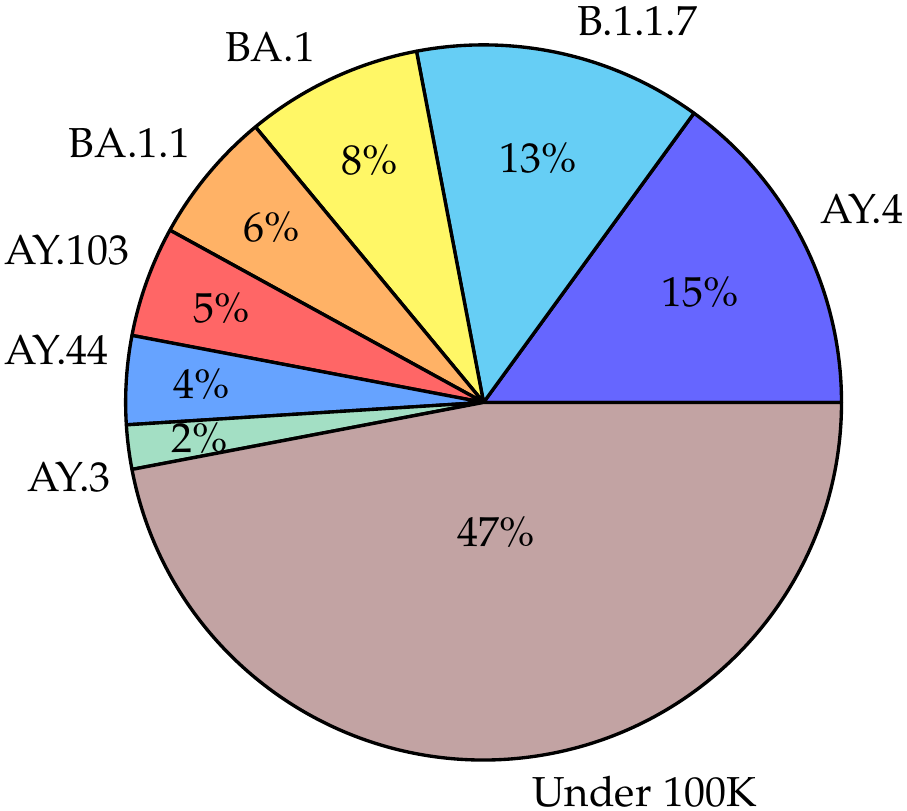
\includegraphics[width=150mm, height=140mm]{pie.png}
			\captionof{figure}{Lineage distribution w.r.t. number of samples}
		\end{center}\vspace{1cm}
		\section*{Main objectives}
		\begin{itemize}
			\item Identification of mutation patterns within single lineages and association rules
			\item Clade discovery
		\end{itemize}
		
		%----------------------------------------------------------------------------------------
		%	MATERIALS AND METHODS
		%----------------------------------------------------------------------------------------
		
		\section*{Methods: Association Rule Mining}
		
		Consider each sample as a \textquotedblleft transaction\textquotedblright$\,$that contains certain items (i.e., mutations). We provide some definitions:
		\begin{itemize}
			\item \textbf{Association rule:} An expression $X$ $\rightarrow$ $Y$, where $X$ and $Y$ are disjoint mutation subsets\cite{arules}. 
			\item \textbf{Support:} The support of a subset of mutations \textit{X}, denoted by $sup(X)$, is the number of transactions (or samples) in a transaction dataset \textbf{D} that contain \textit{X}. 
			\item \textbf{Confidence:} The confidence of a rule is an estimate of the conditional probability that a transaction contains $Y$ given that it contains $X$.
			\begin{align*}
				conf(X \rightarrow Y) = P(Y|X) = \frac{P(X,Y)}{P(X)} = \frac{sup(X,Y)}{sup(X)}
			\end{align*}
			Confidence can be a misleading metric in some cases, it is mostly used for filtering very unlikely rules, but not for assessing their quality.
			\item \textbf{Lift:} Ratio of the observed joint probability of $X$ and $Y$ to the expected joint probability if they were statistically independent.
			\begin{align*}
				lift(X \rightarrow Y) = \frac{P(X,Y)}{P(X)\cdot P(Y)} = \frac{conf(X\rightarrow Y)\cdot |\mathbf{D}|}{sup(Y)}
			\end{align*}
		\end{itemize}
		
		\section*{Pattern recognition within single lineages}
		We decided to study subsets of individual lineages. It is important to note that we performed a repeated sampling of 10K transactions, and the results are consistent throughout all samplings, except for negligible differences. We performed hierarchical clustering on all the features with Ward linkage and chose an appropriate number of clusters. Figure 2 shows the pairs plot (first four PCs) colored by clusters, and Figure 3 shows the dendrogram for AY.103. 
		\begin{center}\vspace{1cm}
			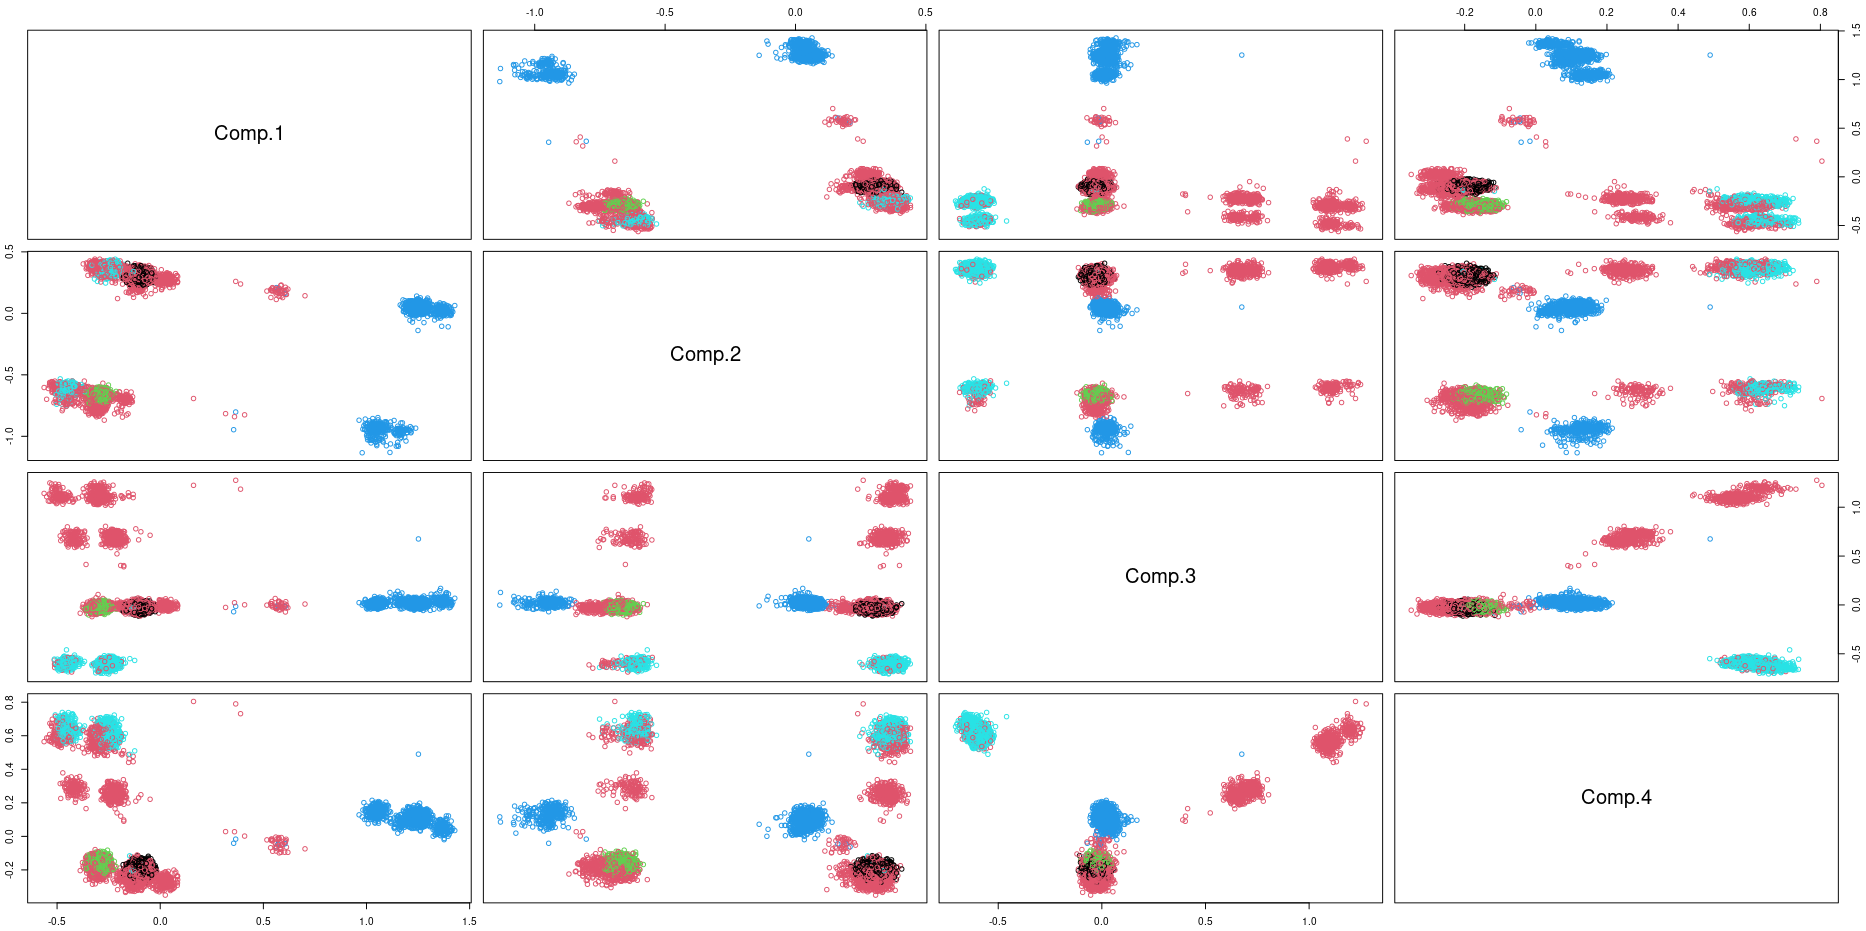
\includegraphics[width=200mm, height=110mm]{pairs2.png}
			\captionof{figure}{Pairs plot colored by cluster. Clustering has captured what we can assess by eye, although the data is high-dimensional}
			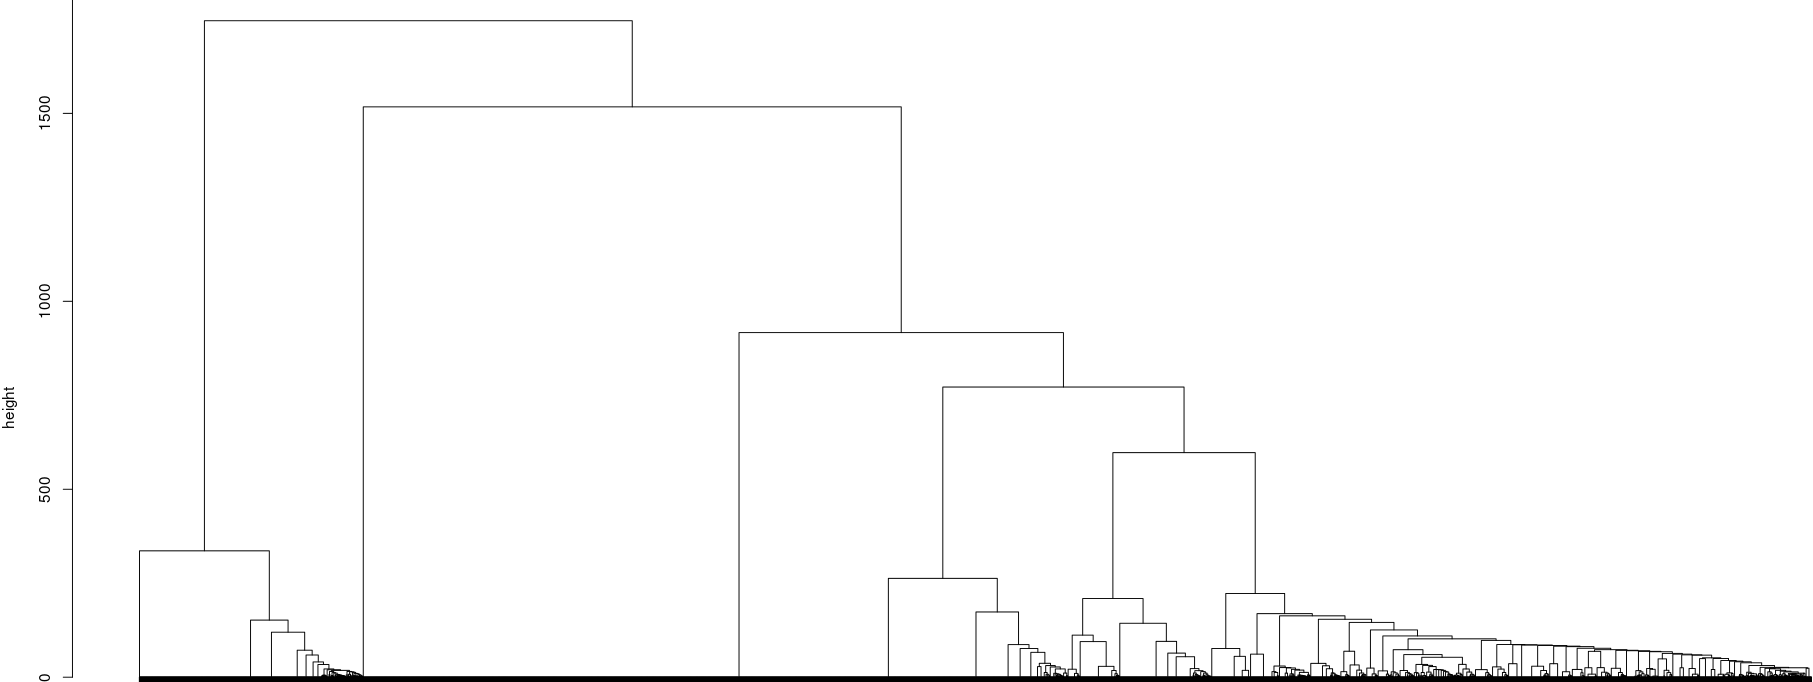
\includegraphics[width=170mm, height=80mm]{dendrogram.png}
			\captionof{figure}{Dendrogram for AY.103 with Ward linkage. Choosing five balanced clusters we suspect there might be subpatterns within the lineage}
		\end{center}\vspace{1cm}
		Figure 4 shows a comparison of the mutation frequency barplots between AY.103 and one of its clusters. 

		\begin{center}\vspace{1cm}
			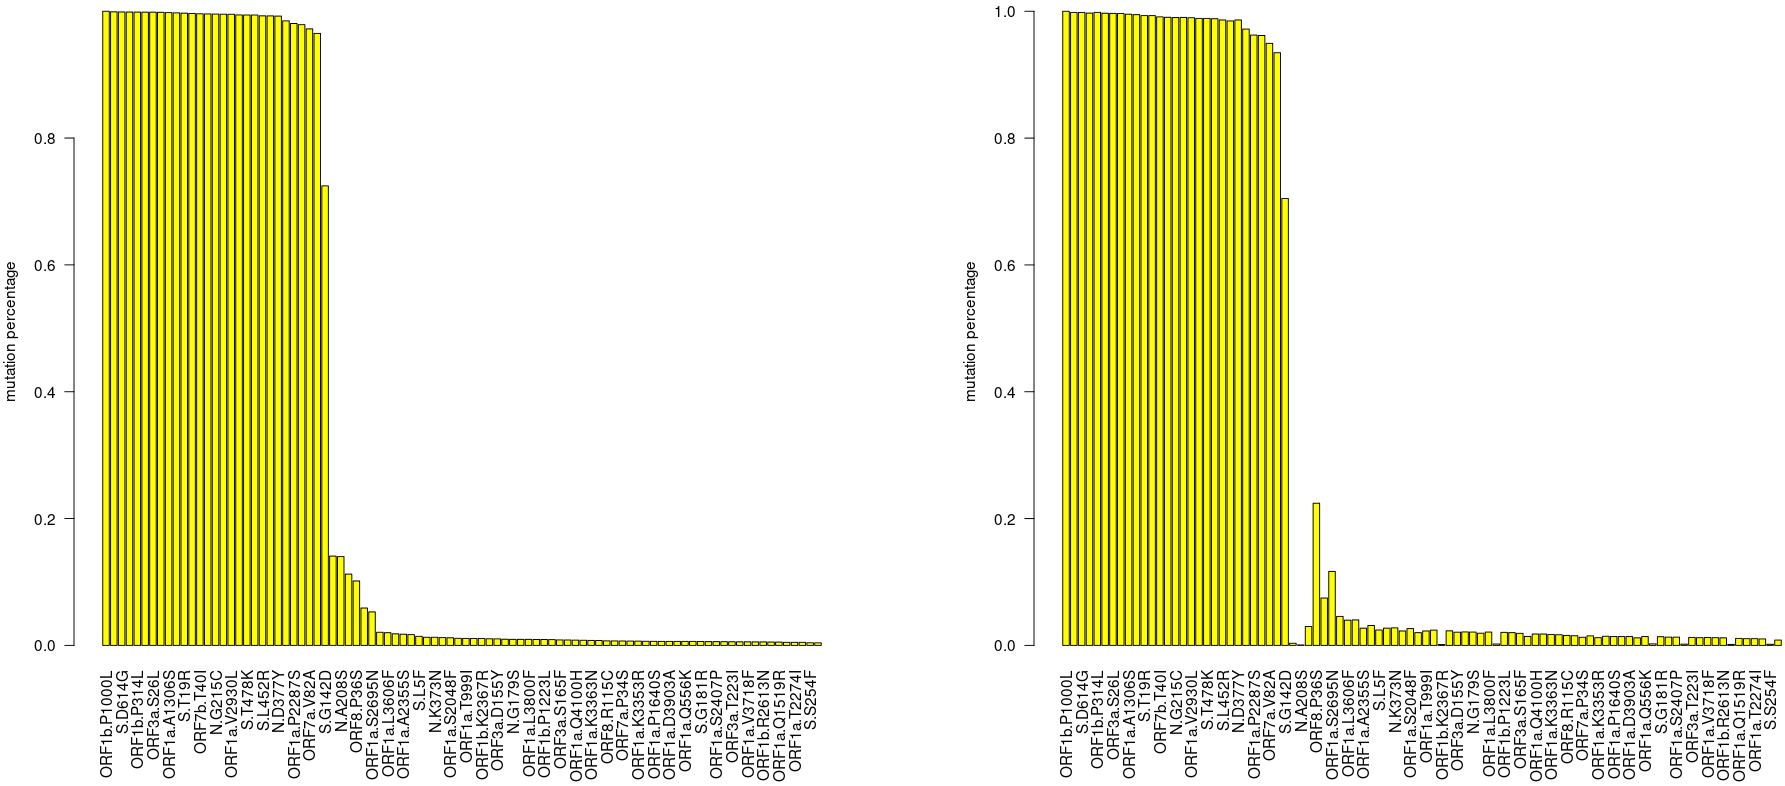
\includegraphics[width=240mm, height=110mm]{comparison2.png}
			\captionof{figure}{Original AY.103 mutation frequency barplot (left) and cluster 1 barplot (right). The mutation spikes in cluster 1 allow us to focus our attention on possibly meaningful rules}
		\end{center}\vspace{1cm}
		The spikes in mutations \{\textit{ORF81a:S2695N}\} and \{\textit{ORF8:P36S}\} suggest the rule \{\textit{ORF81a:S2695N}\}$\rightarrow$\{\textit{ORF8:P36S}\}.  After rule mining, we find such a rule with high confidence (0.989) and high lift (10.335). So we have exploited the information obtained via clustering and redirected our attention to potentially meaningful rules. The biological interpretation is that the mutations may be synergistic or beneficial to the virus or, more importantly, predominant in lineages generated or related to AY.103. Pairs plot colored by cluster. The three clusters found have an accurate correspondence with the clades
		\section*{Clade discovery}
		Can we apply the previous pipeline to clade discovery? We consider five lineages (belonging to three clades) and randomly extract 1600 samples from each. Table 1 shows the lineages and their corresponding clades.
		\begin{center}\vspace{1cm}
			\renewcommand{\arraystretch}{1.2} % enlarge line spacing
			\begin{tabular}{l l }
				\toprule
				\textbf{Lineages} & \textbf{Clade} \\
				\midrule
				AY.103, AY.4 & 21J (Delta)\\
				B.1.1.7 & 20I (Alpha) \\
				BA.1, BA.1.1 & 21K (Omicron) \\
				\bottomrule
			\end{tabular}
			\captionof{table}{Lineages - clade table}
		\end{center}\vspace{1cm}
		We perform clustering, and the dendrogram suggests three balanced clusters. Figure 5 shows the pairs plot (first four PCs, over 92\% of variability).
		\begin{center}\vspace{1cm}
			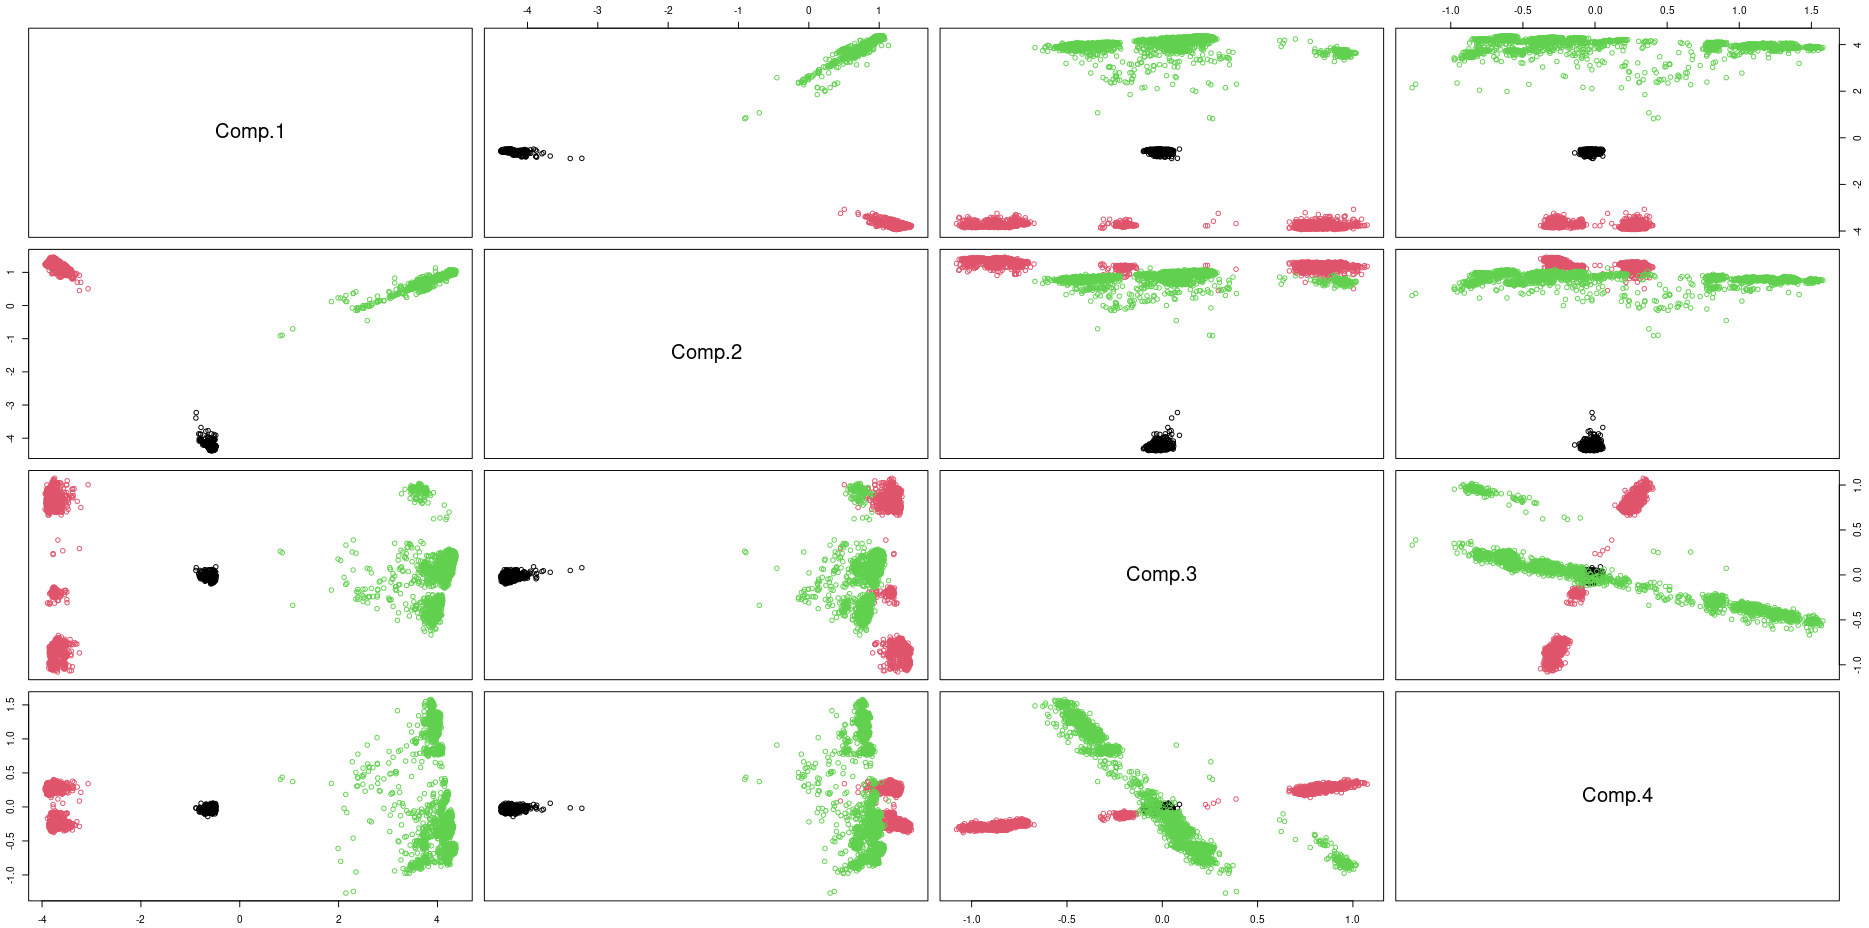
\includegraphics[width=200mm, height=110mm]{pairs3.png}
			\captionof{figure}{Pairs plot colored by cluster. The three clusters found have an almost 	exact correspondence with the clades}
		\end{center}\vspace{1cm}
		
		Our clustering has an almost perfect correspondence with the real clades (the coloring by clade shows an almost identical plot). Therefore, it is reasonable to assume that with more sophisticated techniques, we could apply this pipeline to lineages, which are more fine-grained than clades.
		
		\section*{Conclusion}
		
		
		We have shown that standard techniques such as clustering and association rules can successfully exploit the large amount of data available. For example, smaller datasets, the case with any other virus, would have yielded poor results because of the lack of large-scale random sampling. We found non-trivial mutation patterns because of the reduction of the rule search space via the information provided by clustering. However, these results also have a biological interpretation; mutations tend to appear in pairs, possibly because of synergy between them (i.e., beneficial effect on the virus). Finally, our analysis suggests a data-driven lineage discovery method since clade discovery was successful.
		
		\section*{Forthcoming Research}
		
		Future research focuses on predicting novel sublineages by studying the mutation pairs (or groups) found via association rules. Another unexplored aspect of the data is their functional nature; each sample has the date of sampling, and the analysis of the growth rates of single mutations within lineages may aid in the study of the evolution of new sublineages, such would be the case of the latest Omicron variant, lineage BA.5.
		\begin{thebibliography}{99} 
			\bibitem{arules}
Agrawal, Rakesh, Imieliński, and Swami. "Mining association rules between sets of items in large databases." In Proceedings of the 1993 ACM SIGMOD international conference on Management of data, pp. 207-216. 1993.
		\end{thebibliography}
	\end{multicols}
\end{document}